\documentclass[10pt,a4paper]{article}

\usepackage[a4paper, top=20mm, bottom=16mm, left=18mm, right=18mm]{geometry}
\usepackage{palatino}
\usepackage[T1]{fontenc}
\usepackage[utf8]{inputenc}
\usepackage{microtype}
\usepackage{xcolor}
\usepackage{booktabs}
\usepackage{tabularx}
\usepackage{array}
\usepackage{enumitem}
\usepackage{titlesec}
\usepackage{fancyhdr}
\usepackage{parskip}
\usepackage{mdframed}
\usepackage[hidelinks]{hyperref}
\usepackage{tikz}
\usetikzlibrary{shapes.geometric, arrows.meta, positioning, fit, backgrounds, calc}
\usepackage{etoolbox}
\makeatletter
\patchcmd{\ttlh@hang}{\parindent\z@}{\parindent\z@\leavevmode}{}{}
\patchcmd{\ttlh@hang}{\noindent}{}{}{}
\makeatother

% --- Colors ---
\definecolor{traceblue}{HTML}{1A3C5E}
\definecolor{traceorange}{HTML}{E87722}
\definecolor{tracegreen}{HTML}{16A34A}
\definecolor{tracepurple}{HTML}{7C3AED}
\definecolor{tracered}{HTML}{DC2626}
\definecolor{l0col}{HTML}{2563EB}
\definecolor{l1col}{HTML}{059669}
\definecolor{l2col}{HTML}{EA580C}
\definecolor{l3col}{HTML}{7C3AED}
\definecolor{l4col}{HTML}{DC2626}

% --- Section formatting ---
\titleformat{\section}{\color{traceblue}\large\bfseries}{}{0em}{}[\color{traceorange}\rule{\linewidth}{1.2pt}]
\titlespacing*{\section}{0pt}{8pt}{4pt}
\titleformat{\subsection}{\color{traceblue}\normalsize\bfseries}{}{0em}{}
\titlespacing*{\subsection}{0pt}{6pt}{2pt}

% --- Header / Footer ---
\pagestyle{fancy}
\fancyhf{}
\renewcommand{\headrulewidth}{0pt}
\fancyhead[L]{\small\color{traceblue}\textbf{TRACE.ai} \quad\textcolor{gray}{Technical Architecture}}
\fancyhead[R]{\small\color{traceblue}iDEA 2.0 \textbullet{} PS3 \textbullet{} NamoFans}
\fancyfoot[C]{\small\color{gray}\thepage}

% --- List and table setup ---
\setlist[itemize]{itemsep=1pt, topsep=2pt, parsep=0pt, leftmargin=12pt}
\setlist[enumerate]{itemsep=1pt, topsep=2pt, parsep=0pt, leftmargin=14pt}
\newcolumntype{L}[1]{>{\raggedright\arraybackslash}p{#1}}
\setlength{\parskip}{3pt}

% ============================================================
\begin{document}

% ---- Title block ----
\begin{tikzpicture}[remember picture, overlay]
  \fill[traceblue] (current page.north west) rectangle ([yshift=-20mm]current page.north east);
\end{tikzpicture}

\vspace*{-4mm}
{\color{white}\Large\textbf{TRACE.ai}}\hfill{\color{white!80!traceblue}\small Transaction Risk Analysis and Compliance Engine}

\vspace{1mm}
{\color{traceorange}\footnotesize\textbf{iDEA Hackathon 2.0 \textbullet{} PSBs Hackathon Series 2026 \textbullet{} Union Bank of India \textbullet{} PS3}}

\vspace{0.5mm}
{\color{white!70!traceblue}\footnotesize Team \textbf{NamoFans} \textbullet{} IIT Kharagpur \textbullet{} Animesh Raj \textbullet{} Devansh Gupta \textbullet{} Prem Agarwal \textbullet{} MD.~Faizan Khan}

\vspace{6mm}

% ===========================
%  PAGE 1
% ===========================

\section{System Overview}

TRACE.ai is structured as five independent layers, each exposing a clean interface to the next. No layer imports the internals of another, allowing any module to be replaced independently. The system ingests synthetic banking transaction data (IBM AMLSim), models it as a directed graph, runs four fraud detection signals in parallel, fuses their scores, and serves results to a React 3D dashboard over FastAPI and WebSocket.

\section{Architecture Diagram}

\begin{figure}[h]
\centering
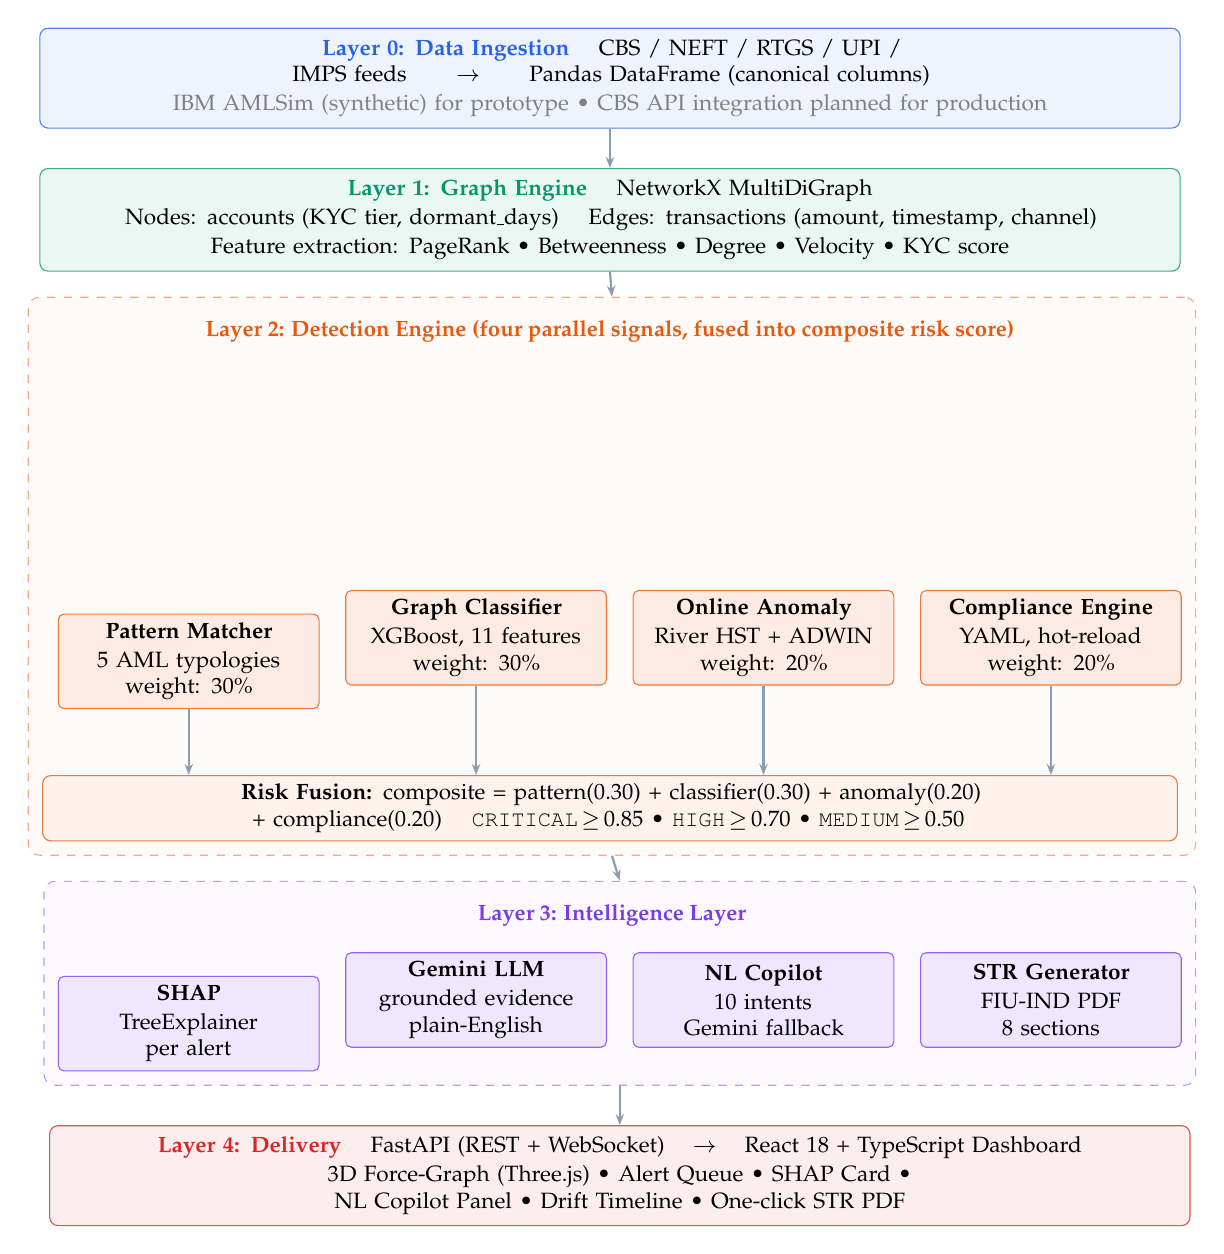
\begin{tikzpicture}[
  font=\footnotesize,
  layerbox/.style={draw=#1!80, fill=#1!8, rounded corners=3pt, text width=14.2cm,
                   minimum height=9mm, align=center, inner sep=4pt},
  signalbox/.style={draw=#1!80, fill=#1!12, rounded corners=2pt, text width=3.1cm,
                    minimum height=12mm, align=center, inner sep=3pt},
  fusionbox/.style={draw=l2col!80, fill=l2col!8, rounded corners=3pt, text width=14.2cm,
                    minimum height=7mm, align=center, inner sep=3pt},
  arr/.style={-{Stealth[length=4pt]}, line width=0.8pt, color=traceblue!50},
  lbl/.style={font=\scriptsize\bfseries\sffamily, rotate=90, text=white, anchor=center},
  strip/.style={fill=#1, rounded corners=1pt, minimum width=5mm},
]

% Layer 0
\node[layerbox=l0col] (L0) at (0,0)
  {\textbf{\color{l0col}Layer 0: Data Ingestion} \quad
   CBS / NEFT / RTGS / UPI / IMPS feeds $\;\to\;$ Pandas DataFrame (canonical columns)\\[1pt]
   {\color{gray}IBM AMLSim (synthetic) for prototype \textbullet{} CBS API integration planned for production}};

% Layer 1
\node[layerbox=l1col, below=5mm of L0] (L1)
  {\textbf{\color{l1col}Layer 1: Graph Engine} \quad
   NetworkX MultiDiGraph\\[1pt]
   Nodes: accounts (KYC tier, dormant\_days) \quad
   Edges: transactions (amount, timestamp, channel)\\[1pt]
   Feature extraction: PageRank \textbullet{} Betweenness \textbullet{} Degree \textbullet{} Velocity \textbullet{} KYC score};

% Layer 2 label
\node[font=\footnotesize\bfseries, color=l2col, below=5mm of L1, anchor=north] (L2lbl)
  {Layer 2: Detection Engine (four parallel signals, fused into composite risk score)};

% Four signal boxes
\node[signalbox=l2col, below=3mm of L2lbl.south, anchor=north] (PA) at (-5.35,-6.5)
  {\textbf{Pattern Matcher}\\[1pt] 5 AML typologies\\weight: 30\%};
\node[signalbox=l2col, anchor=north] (GC) at (-1.7,-6.5)
  {\textbf{Graph Classifier}\\[1pt] XGBoost, 11 features\\weight: 30\%};
\node[signalbox=l2col, anchor=north] (OA) at (1.95,-6.5)
  {\textbf{Online Anomaly}\\[1pt] River HST + ADWIN\\weight: 20\%};
\node[signalbox=l2col, anchor=north] (CE) at (5.6,-6.5)
  {\textbf{Compliance Engine}\\[1pt] YAML, hot-reload\\weight: 20\%};

% Risk fusion
\node[fusionbox, below=4mm of PA.south, anchor=north] (RF) at (0,-8.45)
  {\textbf{Risk Fusion:} composite = pattern(0.30) + classifier(0.30) + anomaly(0.20) + compliance(0.20)
   \quad \texttt{CRITICAL}$\,\geq\,$0.85 \textbullet{} \texttt{HIGH}$\,\geq\,$0.70 \textbullet{} \texttt{MEDIUM}$\,\geq\,$0.50};

% Bounding box for Layer 2
\begin{scope}[on background layer]
  \node[draw=l2col!50, fill=l2col!3, rounded corners=4pt, dashed, inner sep=5pt,
        fit=(L2lbl)(PA)(GC)(OA)(CE)(RF)] (L2box) {};
\end{scope}

% Layer 3
\node[below=5mm of L2box] (L3lbl)
  [font=\footnotesize\bfseries, color=l3col] {Layer 3: Intelligence Layer};

\node[signalbox=l3col, below=3mm of L3lbl.south, anchor=north] (SH) at (-5.35,-11.1)
  {\textbf{SHAP}\\[1pt] TreeExplainer\\per alert};
\node[signalbox=l3col, anchor=north] (GE) at (-1.7,-11.1)
  {\textbf{Gemini LLM}\\[1pt] grounded evidence\\plain-English};
\node[signalbox=l3col, anchor=north] (CO) at (1.95,-11.1)
  {\textbf{NL Copilot}\\[1pt] 10 intents\\Gemini fallback};
\node[signalbox=l3col, anchor=north] (ST) at (5.6,-11.1)
  {\textbf{STR Generator}\\[1pt] FIU-IND PDF\\8 sections};

\begin{scope}[on background layer]
  \node[draw=l3col!50, fill=l3col!3, rounded corners=4pt, dashed, inner sep=5pt,
        fit=(L3lbl)(SH)(GE)(CO)(ST)] (L3box) {};
\end{scope}

% Layer 4
\node[layerbox=l4col, below=5mm of L3box] (L4)
  {\textbf{\color{l4col}Layer 4: Delivery} \quad
   FastAPI (REST + WebSocket) $\;\to\;$ React 18 + TypeScript Dashboard\\[1pt]
   3D Force-Graph (Three.js) \textbullet{} Alert Queue \textbullet{} SHAP Card \textbullet{} NL Copilot Panel
   \textbullet{} Drift Timeline \textbullet{} One-click STR PDF};

% Arrows
\draw[arr] (L0.south) -- (L1.north);
\draw[arr] (L1.south) -- (L2box.north);
\foreach \s in {PA,GC,OA,CE} { \draw[arr] (\s.south) -- (\s.south |- RF.north); }
\draw[arr] (L2box.south) -- (L3box.north);
\draw[arr] (L3box.south) -- (L4.north);

\end{tikzpicture}
\caption{TRACE.ai five-layer architecture with one-directional data flow.}
\end{figure}

\newpage

% ===========================
%  PAGE 2
% ===========================

\section{Technology Stack}

\begin{tabularx}{\linewidth}{L{1.7cm} L{4.0cm} X}
\toprule
\textbf{Layer} & \textbf{Technology} & \textbf{Why This Choice} \\
\midrule
Data & IBM AMLSim + Pandas 2.0 & Realistic synthetic Indian banking data; reproducible generation; no real CBS required. \\[1pt]
Graph Engine & NetworkX 3.3 MultiDiGraph & Sufficient for 500 to 5,000 account prototype; no external database. Neo4j GDS targeted for production. \\[1pt]
Graph Features & scikit-learn + NetworkX & 11 features (degree, PageRank, betweenness, velocity, KYC score, dormancy) capturing structure a GNN would learn from raw adjacency. \\[1pt]
ML Classifier & XGBoost 2.1.4 & AUC above 0.99 on synthetic data; natively supported by SHAP TreeExplainer; interpretable for compliance. \\[1pt]
Online Anomaly & River 0.23.0 (HST + ADWIN) & Per-account streaming baselines at sub-millisecond latency; no batch retraining needed. \\[1pt]
Compliance & PyYAML + watchdog & Hot-reload YAML rules without restart; compliance teams update rules without engineering. \\[1pt]
LLM & Gemini 2.5 Flash (Vertex AI) & GCP credits available; grounded evidence block prevents hallucination; fast for structured prompts. \\[1pt]
STR PDF & ReportLab 4.1 & Programmatic 8-section A4 PDF in FIU-IND format with tables, fund trail diagram, and risk charts. \\[1pt]
Backend & FastAPI 0.110 + WebSocket & Asynchronous; WebSocket for live alert streaming; OpenAPI docs auto-generated. \\[1pt]
Frontend & React 18 + TypeScript + Vite & Type-safe hooks architecture; Vite proxy for local dev; compiled SPA served by FastAPI. \\[1pt]
3D Graph & react-force-graph-3d + Three.js & GPU-accelerated force-directed graph; nodes glow by risk level in real time. \\[1pt]
Deploy & GCP Cloud Run + Docker & Single container; no CORS configuration; scales to zero when idle; demo data baked in at build time. \\
\bottomrule
\end{tabularx}

\section{Key Technical Decisions}

\begin{itemize}
  \item \textbf{XGBoost instead of a full Temporal GNN.} Phase 1 described ChronoWave-GNN. For the prototype, XGBoost on graph-structural features is the correct approach: PyTorch Geometric TGN requires more data and compute. SHAP TreeExplainer provides attribution equivalent to GNNExplainer. A trained TGN checkpoint (\texttt{models/tgn\_classifier.pt}, AUC 0.72) is included; the trade-off is documented in \texttt{MODEL\_CARD.md}.
  \item \textbf{NetworkX instead of Neo4j.} Adequate for 500 to 5,000 accounts; eliminates an external dependency. The graph builder (\texttt{src/trace/graph/builder.py}) can be swapped for a Neo4j connector without touching detection or intelligence layers (ADR-0003 in \texttt{DECISIONS.md}).
  \item \textbf{Compliance rules as YAML, not code.} RBI Master Directions change frequently. YAML hot-reload with watchdog lets compliance teams update rules without an engineering deployment. A new circular takes effect within 5 seconds.
  \item \textbf{Single-container deployment.} FastAPI serves the React SPA as StaticFiles. One Cloud Run URL; no CORS configuration. Demo data is seeded at image build time so the container starts cold with all alerts pre-populated.
\end{itemize}

\section{Known Limitations}

\begin{itemize}
  \item \textbf{Synthetic data only.} Metrics are on IBM AMLSim data. Real-bank performance requires retraining on CBS feeds.
  \item \textbf{Batch graph, not real-time stream.} Production requires a Kafka consumer for live CBS event ingestion.
  \item \textbf{NetworkX at prototype scale.} Not suitable for millions of accounts; Neo4j GDS is the production path.
  \item \textbf{No user authentication.} Dashboard is publicly accessible (POC). Production requires LDAP/SSO.
  \item \textbf{FIU-IND STR format is simulated.} The PDF follows the 8-section structure but is not legally compliant and has no digital signature.
  \item \textbf{5 fraud typologies in POC.} Production requires 15 to 20. Adding a new typology requires only a new module in \texttt{src/trace/detection/patterns/}.
\end{itemize}

\vspace{4mm}
\noindent\colorbox{traceblue!8}{\parbox{\dimexpr\linewidth-10pt\relax}{\footnotesize\color{traceblue}\sloppy
\textbf{Live:} \url{https://trace-ai-4xnj5ovp4a-uc.a.run.app} \quad
\textbf{Repo:} \url{https://github.com/wildcraft958/namofans-trace-ai}
}}

\end{document}
